\chapter{Análisis espectrales: resultados numéricos}

\begin{itemize}
	\item Usando la transformada discreta de Fourier
	(c.f. \ref{sec: TDF}), el espectro de
	una señal $x$ es la gráfica de las frecuencias
	enteras \TODO{ref}
	versus los coeficientes
	$\tau_{n}(x)$ (c.f. \TODO{ref}).
	
	\item Si, para hacer un análisis espectral, se usan
	las ideas propuestas en 
	la sección
	\ref{sec: metodologia para realizar un analisis espectral que considere frecuencias arbitrarias}, entonces, dado un rango de frecuencias 
	$\omega$,
	el espectro de $x$, consiste de la gráfica de 
	las frecuencias $\omega$ versus	
	los coeficientes
	$\sigma_{n}(x, \omega)$ 
\end{itemize}


\begin{figure}[H]
	\sidecaption{
	Ejemplo de los espectros resultantes
	de los dos métodos de análisis.
	\label{fig: espectro 1 }
	}
	\centering
	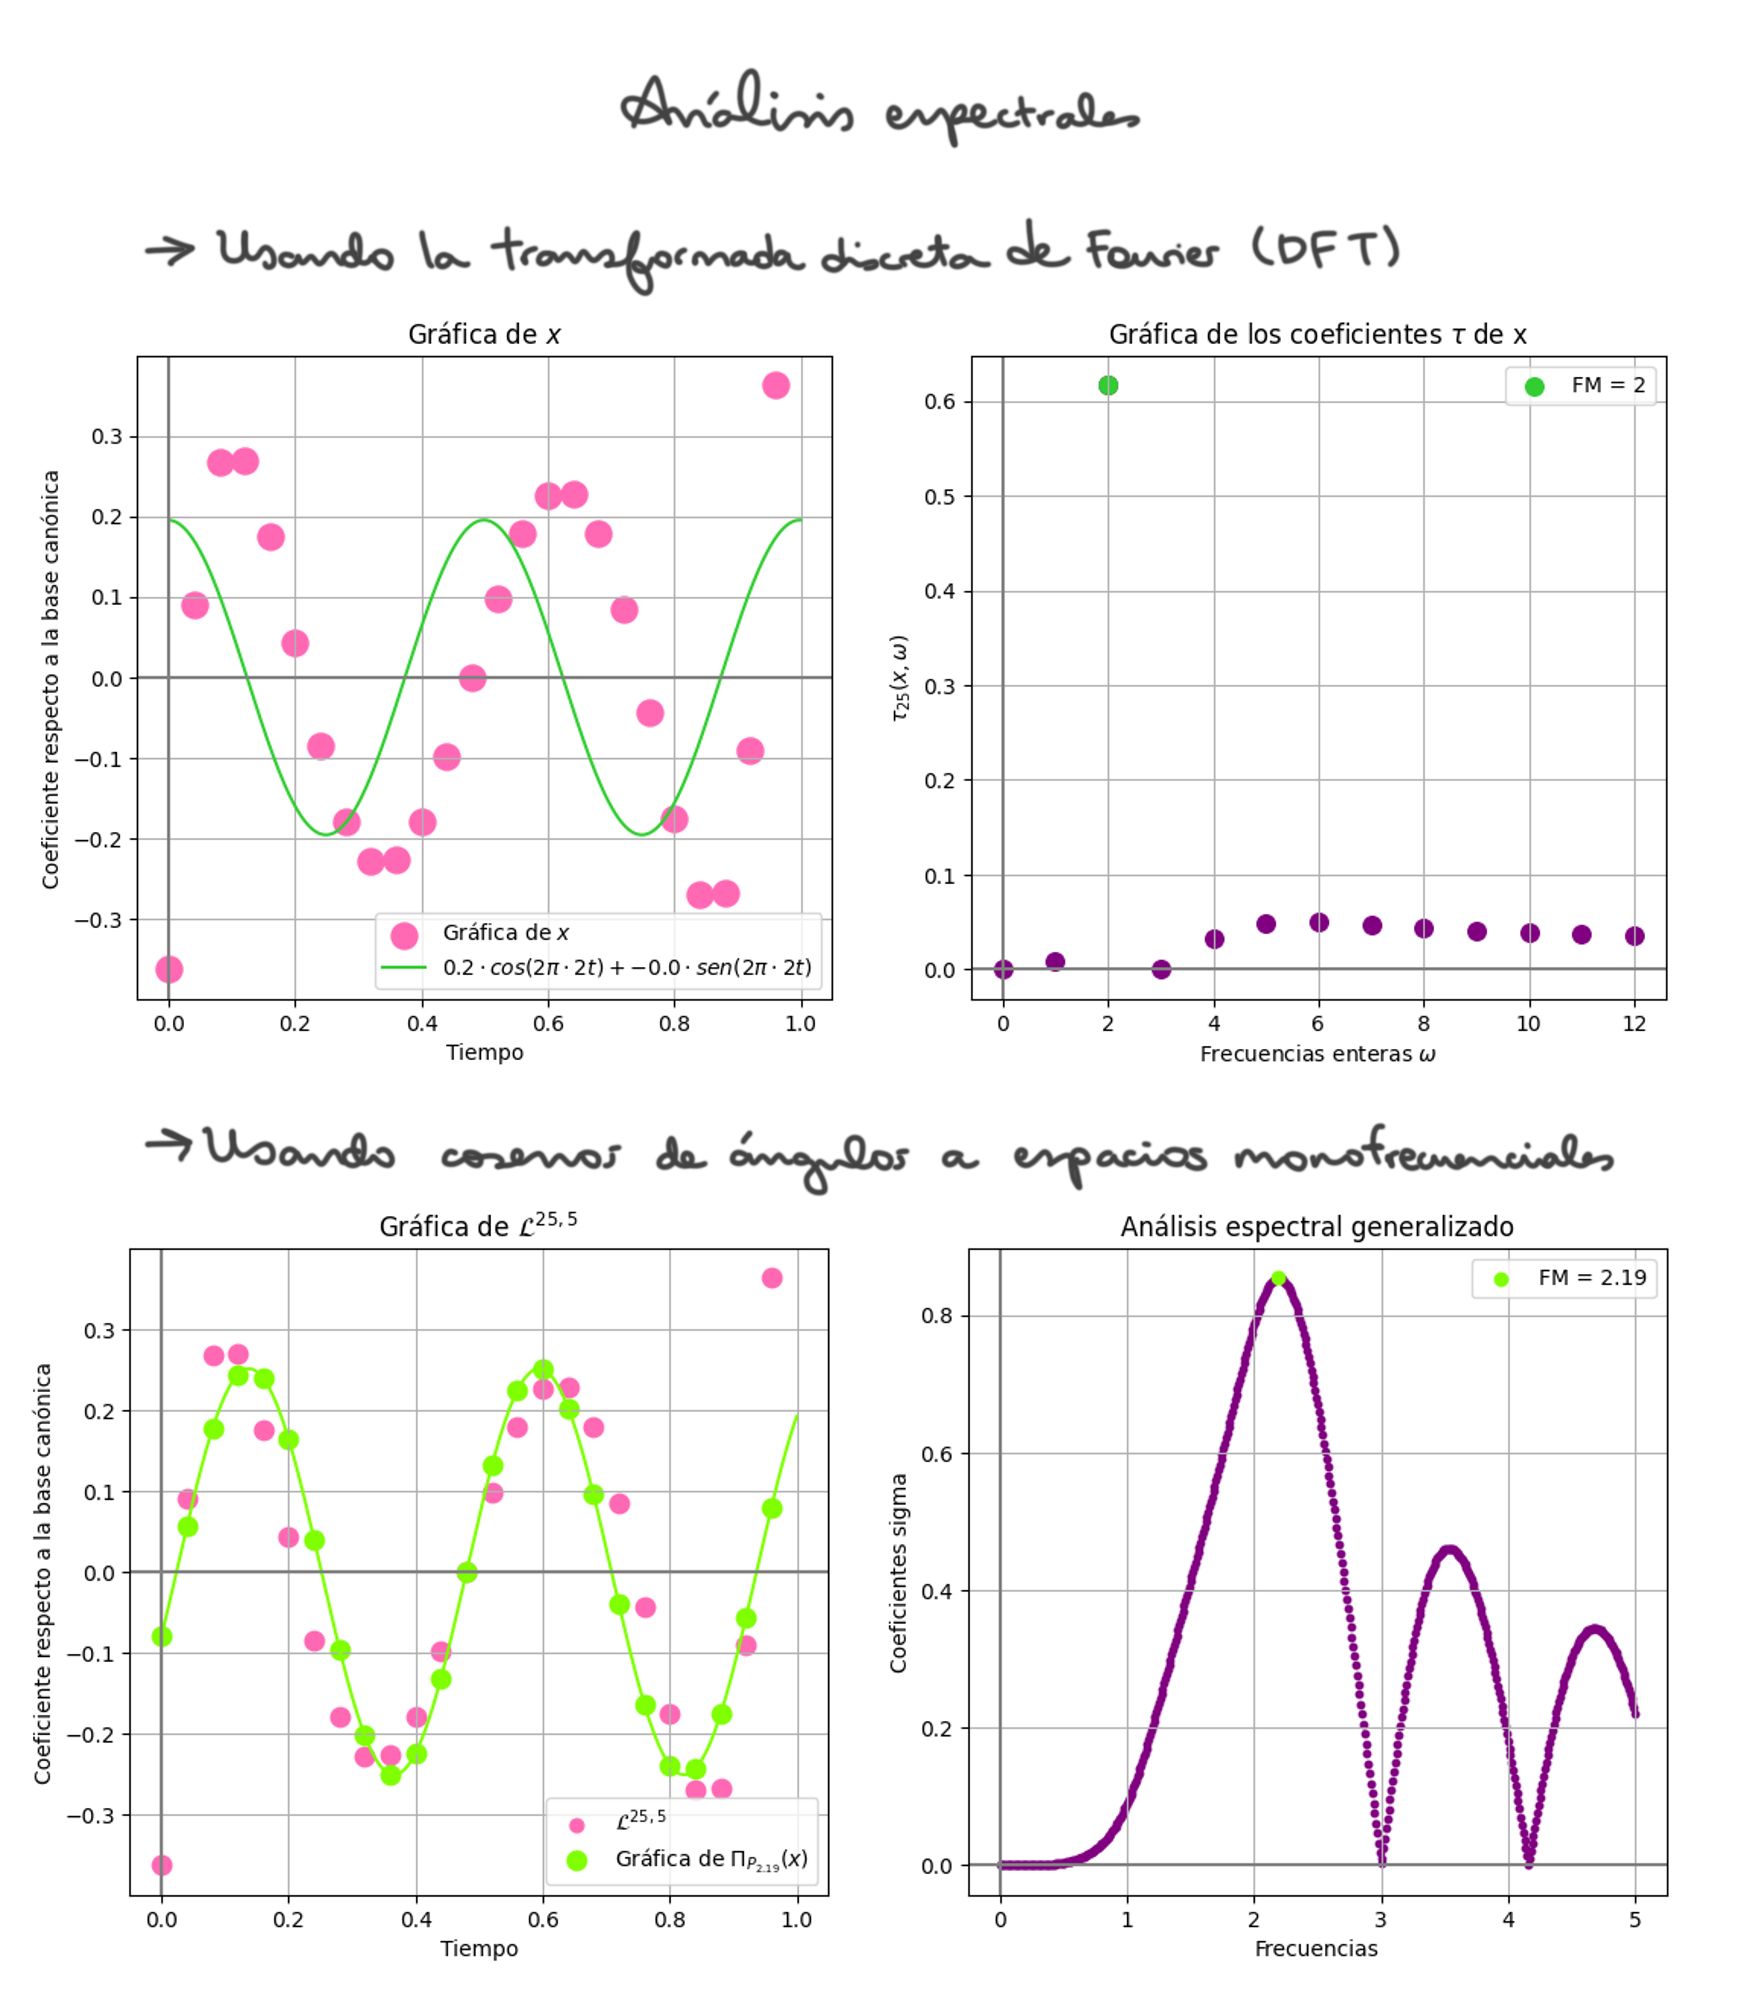
\includegraphics[scale = 1]{ejemplo_analisisEspectrales} 
\end{figure}	